%%%%%%%%%%%%%%%%%%%%%%%%%%%%%%%%%%%%%%%%%%%%%%%%%%%%%%%%%%%%%%%%%%%%%%%%%
%\begin{figure}[p]
% \begin{center}
%  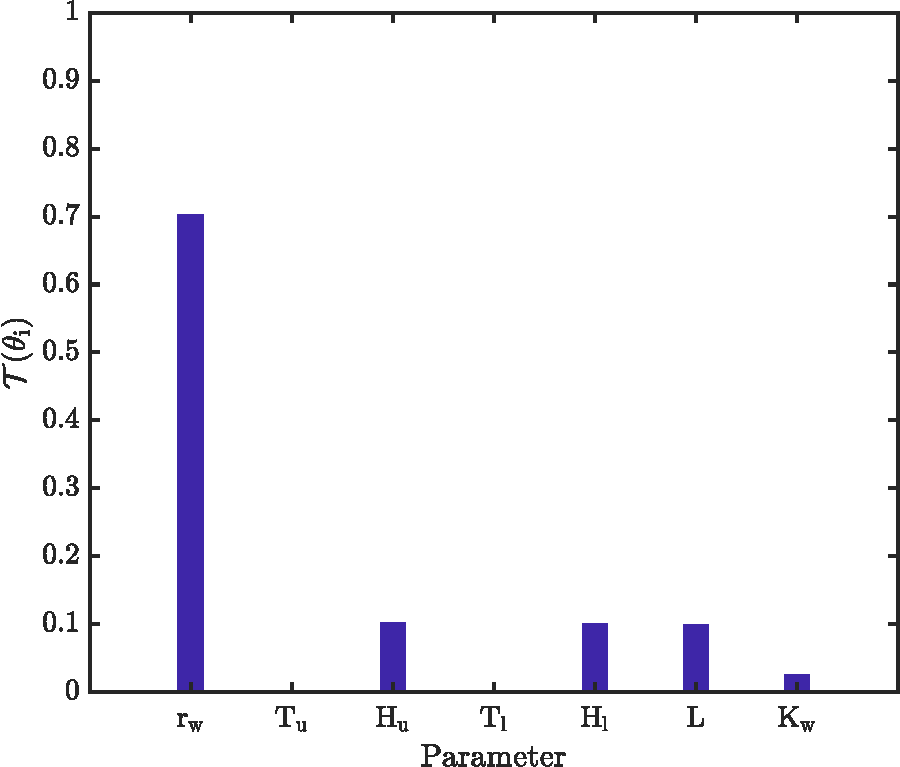
\includegraphics[width=0.70\textwidth]{./Figures/sense_borehole}
%\caption{Sobol' total effect sensitivity index for uncertain parameters in the borehole
%function (Eq.~\ref{eq:bore}).}
%\label{fig:sense_bore}
%\end{center}
%\end{figure}

%\clearpage

%%%%%%%%%%%%%%%%%%%%%%%%%%%%%%%%%%%%%%%%%%%%%%%%%%%%%%%%%%%%%%%%%%%%%%%%%
%\begin{figure}[p]
% \begin{center}
%  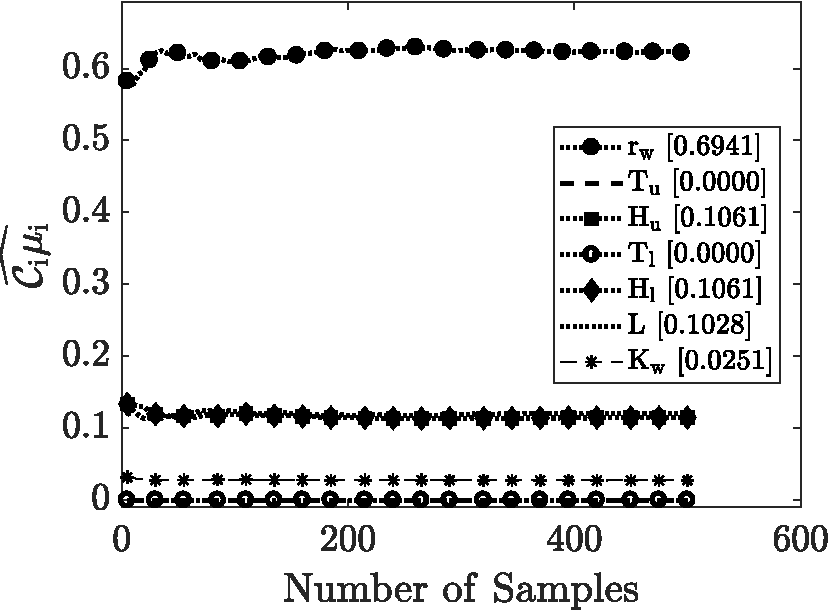
\includegraphics[width=0.70\textwidth]{./Figures/ub_conv_borehole}
%\caption{Estimates of the screening parameter ($\hat{\mathcal{C}_i\mu_i}$) is plotted 
%against number of samples considered for evaluating $\mu_i$. Corresponding estimates
%for the converged Sobol' total effect index ($\mathcal{T}(\theta_i)$) in each case is also included in the
%legend.}
%\label{fig:screen_bore}
%\end{center}
%\end{figure}
%
%\clearpage

%%%%%%%%%%%%%%%%%%%%%%%%%%%%%%%%%%%%%%%%%%%%%%%%%%%%%%%%%%%%%%%%%%%%%%%%%
%\begin{figure}[p]
% \begin{center}
%  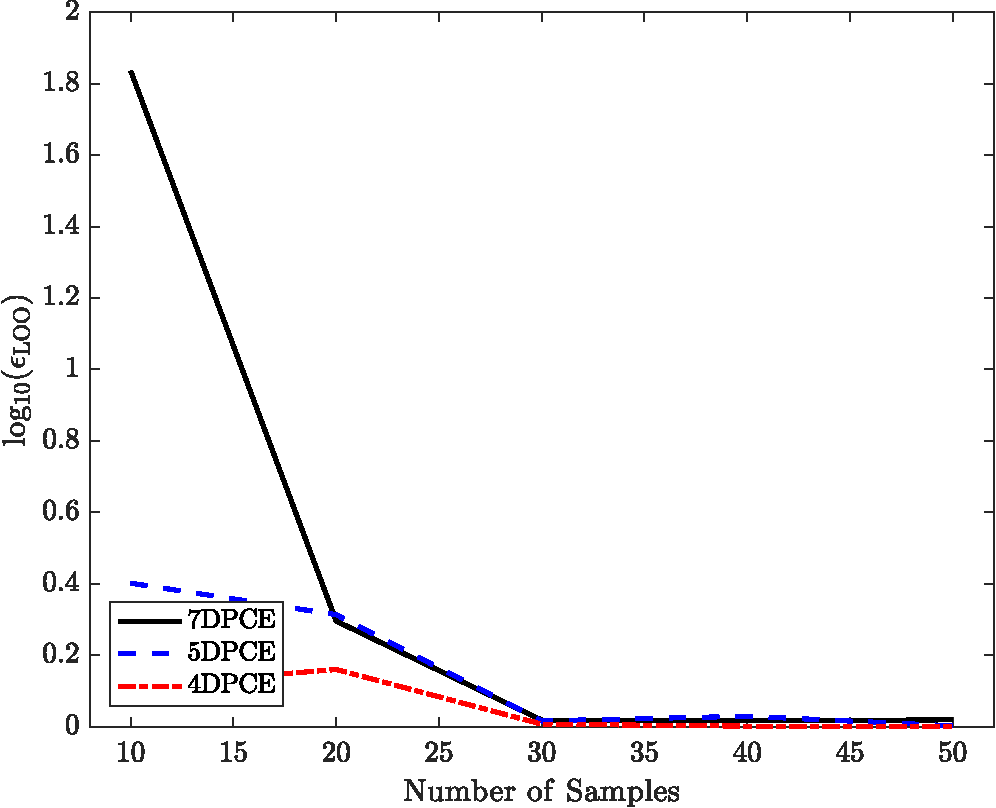
\includegraphics[width=0.70\textwidth]{./Figures/err_samples_borehole}
%\caption{A comparison of order of the leave-one-out-error 
%($\epsilon_{\mbox{\tiny{LOO}}}$) as a function of number of regression samples
%used for constructing the PCE in 4, 5, and 7 dimensions.}
%\label{fig:conv_bore}
%\end{center}
%\end{figure}
%
%\clearpage

%%%%%%%%%%%%%%%%%%%%%%%%%%%%%%%%%%%%%%%%%%%%%%%%%%%%%%%%%%%%%%%%%%%%%%%%%
%\begin{figure}[p]
% \begin{center}
%  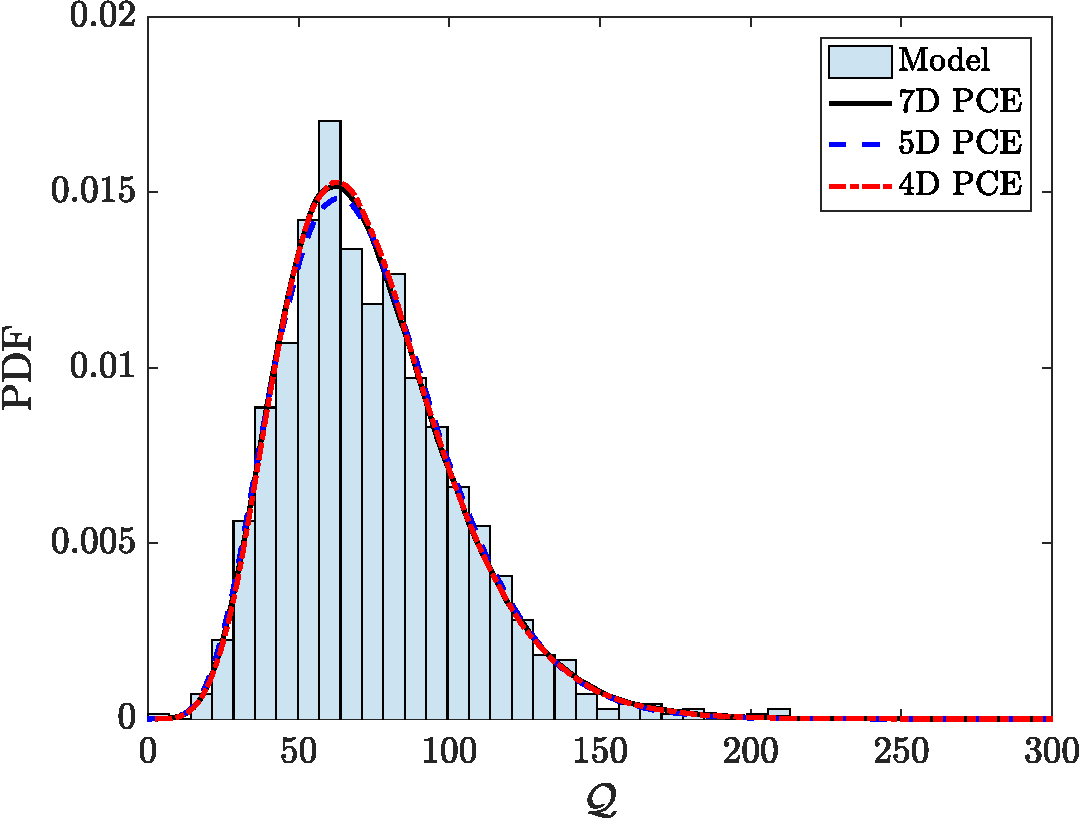
\includegraphics[width=0.70\textwidth]{./Figures/pdf_comp_borehole}
%\caption{A comparison of PDF's of the discharge, $\mathcal{Q}$ as obtained
%by propagating
%parametric uncertainties through the 4D, 5D, and 7D PCE's.These PDF's 
%were obtained using 10$^{6}$ MC samples in the input parameter domain.} 
%\label{fig:pdfcomp_bore}
%\end{center}
%\end{figure}
%
%\clearpage

%%%%%%%%%%%%%%%%%%%%%%%%%%%%%%%%%%%%%%%%%%%%%%%%%%%%%%%%%%%%%%%%%%%%%%%%%
%\begin{figure}[p]
% \begin{center}
%  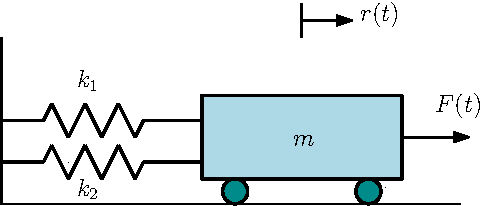
\includegraphics[width=0.70\textwidth]{./Figures/oscillator}
%\caption{Schematic illustration of a non-linear oscillator.}
%\label{fig:pdfcomp_bore}
%\end{center}
%\end{figure}
%
%\clearpage

